\section{Implementation}\label{Implementation}
In this section we will describe how our data has been setup and how our various method have been implemented. Subsection \ref{TET_features} and \ref{TET_historgram_and_distance} will focus on describing how our TET features how we compare them. Subsection \ref{GED} will describe how GED works. Subsection \ref{Metric_Tree_rep} and lastly in subsection \ref{node2vec} and \ref{brute_force} we describe how we implemented node2vec and a brute force comparison method.

\section{TET limitations}
$User(U)  \stackrel{M}{\longrightarrow} Rating(U,M) \stackrel{G}{\longrightarrow} Genre(M,G)$

\subsection{TET Histograms and Distance}
	Comparing the TET can be done in different ways. One of the methods that can be used to find similarity between the TETs is to transform the TETs into histograms and compare these\cite{JAEGER201330}. By counting the number of each type of subTET we can calculate each substructure's percentile distribution for \autoref{fig:Tetekempel}, by dividing the number of subTET in a specific type by the total number of subTETs. The simple TET in \autoref{Eq:TETvector} would give a representation as \autoref{fig:Tethistogram}.
	
	\begin{figure}[H]
		\centering
		\begin{adjustbox}{width=0.5\textwidth}
			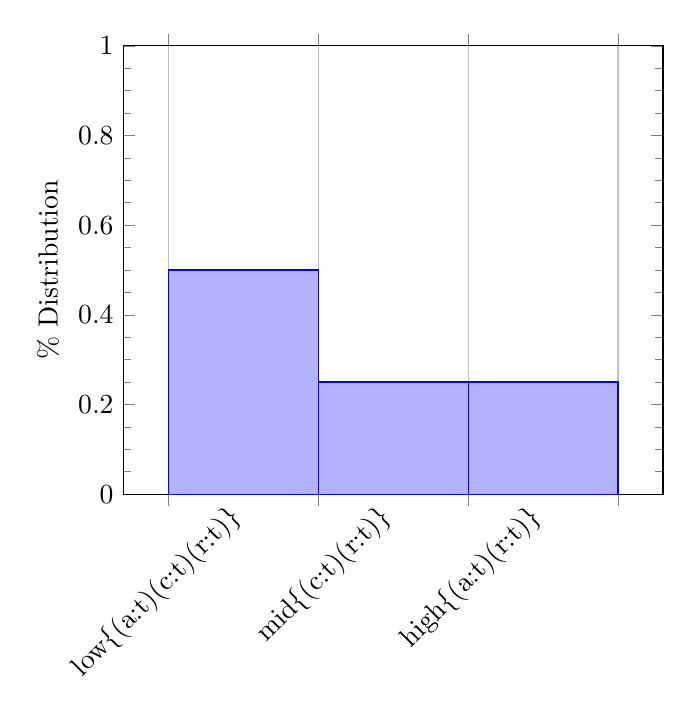
\begin{tikzpicture}
	\begin{axis}[
	ybar interval, 
	ymax=1,ymin=0, 
	minor y tick num = 3,
	ylabel = {\% Distribution},
	symbolic x coords={low\{(a:t)(c:t)(r:t)\}, mid\{(c:t)(r:t)\}, high\{(a:t)(r:t)\}, high\{(y:t)(r:t)\}},
	x tick label style={font=\normalsize, rotate=45, anchor=east},
	]
	\addplot coordinates {(low\{(a:t)(c:t)(r:t)\}, 0.5) (mid\{(c:t)(r:t)\}, 0.25) (high\{(a:t)(r:t)\}, 0.25) (high\{(y:t)(r:t)\}, 0.10)};
	\end{axis}
\end{tikzpicture}

%\begin{tikzpicture}

%\definecolor{bblue}{HTML}{4F81BD}

%\begin{axis}[
%major x tick style = transparent,
%ymin=0,
%bar width=1cm,
%minor y tick num = 3,
%ymajorgrids = true,
%ylabel = {\% distribution},
%symbolic x coords={low\{(a:t)(c:t)(r:t)\}, mid\{(c:t)(r:t)\}, high\{(a:t)(r:t)\}},
%xtick = data,
%x tick label style={font=\normalsize, rotate=45, anchor=east},
%]
%\addplot[ybar , style={bblue,fill=bblue,mark=none}]
%coordinates {(low\{(a:t)(c:t)(r:t)\}, 0.5) (mid\{(c:t)(r:t)\}, 0.25) (high\{(a:t)(r:t)\}, 0.25)};

%\end{axis}
%\end{tikzpicture}
		\end{adjustbox}
		\caption{The TET histogram derived from \autoref{fig:Tetekempel}}
		\label{fig:Tethistogram}
	\end{figure}
	
	By using this representation as a vector we can compare two histograms with simple distance measures as for example manhatten or euclidean distance.
	
	when comparing two histograms, one might have some elements that the other does not have. For any missing element in a histogram we add the value $0$, and we are thereby able to calculate distance for the missing element. A simple example done with manhatten distance can be seen in \autoref{Eq:manhattencomparason}\cite{singh2013k}.
	
	\begin{equation}\label{Eq:manhattencomparason}
	D(\begin{bmatrix}
	x_{1.1} \\
	x_{1.2} \\
	\end{bmatrix},
	\begin{bmatrix}
	x_{2.1} \\
	x_{2.2} \\
	x_{2.3}
	\end{bmatrix})= |x_{1.1} - x_{2.1}| + |x_{1.2} - x_{2.2}| + |0 - x_{2.3}|
	\end{equation}
	
	\autoref{Eq:manhattencomparason} is easily implemented if the vectors are represented as dictionaries. We can then go through the union of dictionary keys from the two dictionaries and return $0$ if a key is not found. The value $0$ will then be used in the calculation. 

\subsection{Graph Edit Distance}\label{Subsec:GED}
As the Graph Edit Distance metric is used in the SimGNN algorithm mentioned in \autoref{AP:SimGNN}, we give a quick explanation of here before continuing with the rest of the appendix.

Graph Edit Distance (GED) is a metric for comparing graphs. The GED of two graphs $a$ and $b$ is a numeric distance value between the graphs. As seen in \autoref{Eq:ged}, the GED is calculated as the fewest number of edits needed in order to transform one graph into the other\cite{Riesen2015}.

\begin{equation}\label{Eq:ged}
 GED(g,g') = \min_{(e_1,e_2 \dots e_k) \in P(g, g') } \sum_{i=1}^k c(e_i)
\end{equation}

In \autoref{Eq:ged} $P(g,g')$ is the set of paths being edited and $c$ is the cost function, measuring the strength of a node edit operation $e_i$\cite{Riesen2015}.

\subsection{Metric Tree}
Because of the datasets size and the linear time it takes to compare one element against all others and the exponential time it would take to compare each element with every other element metric tree approximation can be an option of a stable classifier. 

Metric trees is a group of classifiers that include bk-trees, m-trees, etc. and the implemented metric tree uses the same principles as the ones mentioned. The tree is a collection of nodes bound in a root, the root is itself a node. Each node can be internal or a leaf, if the root is in internal node two random elements in the dataset and splits the dataset around them. The new datasets will be used to create the children of the internal node. An internal node will contain the two elements so that they can be used to search the tree. A leaf contains a bucket of data. The comparisons will still be linear or exponential time dependent on the job but the set of elements smaller and more manageable.

Before the construction of the tree two parameters can be predetermined. The height of the tree will determine the maximum number of groupings or buckets, the groups will grow exponentially with the height of the tree. The second predetermined value is maximum bucket size. These two variables determine when to stop building the tree if a subdataset has less than the maximum bucket size or the node is at the maximal height.

\input{Article/Implementation/Node2vec_imp}
\subsection{Brute force comparison}\label{Subsec:brute_force}
One of the most simple methods of comparing users in data set is to compare all relations one by one. 
In an unweighted graph if there was a relation from a user $A$ to a product $p$ and a relation from user $B$ to $p$ there would be a distance $d$ of 0 between these users assuming that this is the only relation user A and B has. 
A weighted graph the distance would also depend on the relation weight, if $A$ has a relation to $p$ with a weight of 2 and $B$ with a relation to $p$ with a weight of 3, using Manhattan distance there would a distance of 1 between $A$ and $B$. 
This can then be extended to all product relations $P$ as seen in \autoref{eq:manhat}

\begin{equation}\label{eq:manhat}
	d(A,B) = \sum_{i=1}^{P} |A_i - B_i|
\end{equation}
